\begin{frame}[t]
  \frametitle{One-electron problem}
  For $N=1$
  \[ \left[ -\frac{1}{2} \nabla^2 + V(r) \right] \varphi = E \varphi \]
  Separation of variables:
  \[ \varphi(r,\theta,\phi) = R(r)Y(\theta,\phi) \]
  \begin{eqnarray*}
    \text{Angular part} & \emph{Y(\theta,\phi)} & \text{Easy, spherical harmonics} \\
    \text{Radial part} & \emph{R(r)} & \text{Difficult, \alert{our task}}
  \end{eqnarray*}
\end{frame}

\begin{frame}[t]
  \frametitle{One-electron problem}
  \footnotesize
  Angular equation
  \[\frac{1}{\sin{\theta}} \frac{\partial}{\partial \theta} \left( \sin{\theta} \frac{\partial Y}{\partial \theta} \right) + \frac{1}{\sin^2{\theta}} \frac{\partial^2 Y}{\partial \phi^2} = -l(l+1) Y\]
  
  \vspace{-1.6em}
  \pause
  \begin{center}
  \begin{tabular}{c c c c c}
  & & 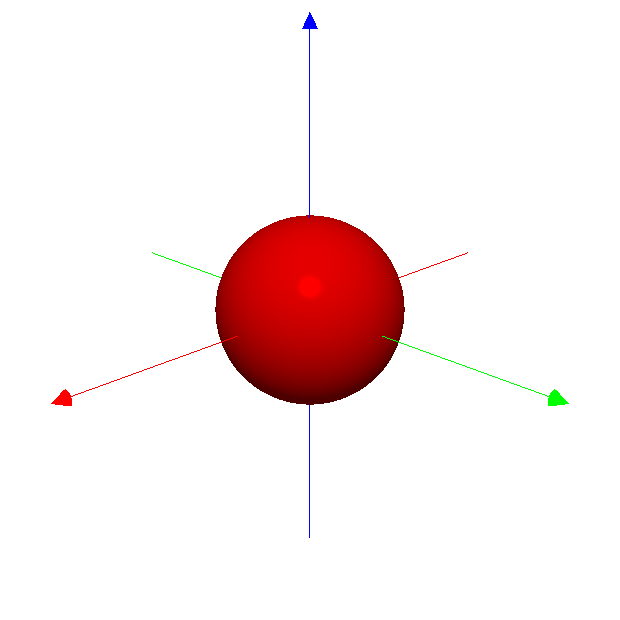
\includegraphics[width=0.15\textwidth,trim={0 3cm 0 -2cm},clip]{00} & & \\
  & 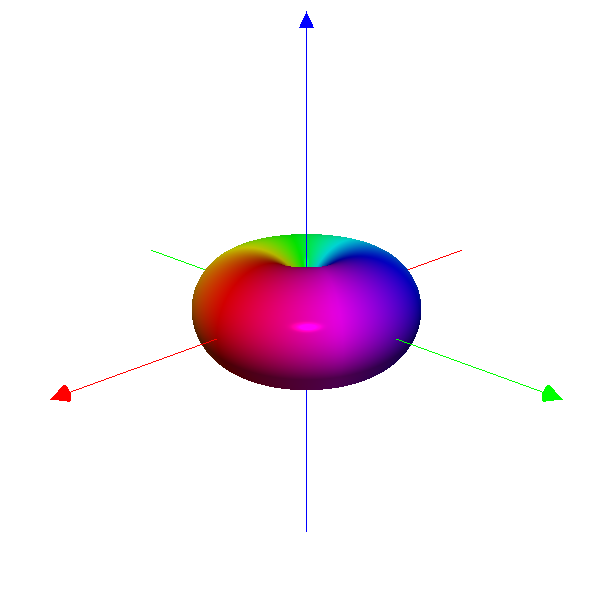
\includegraphics[width=0.15\textwidth,trim={0 3cm 0 -2cm},clip]{1m1} & 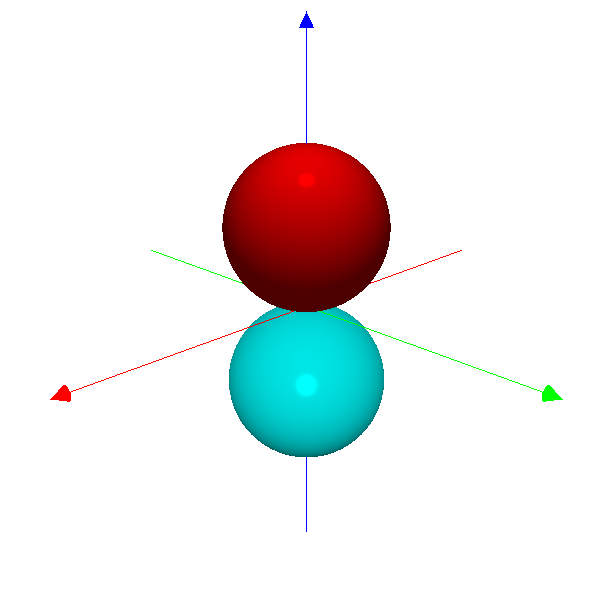
\includegraphics[width=0.15\textwidth,trim={0 3cm 0 -2cm},clip]{10} & 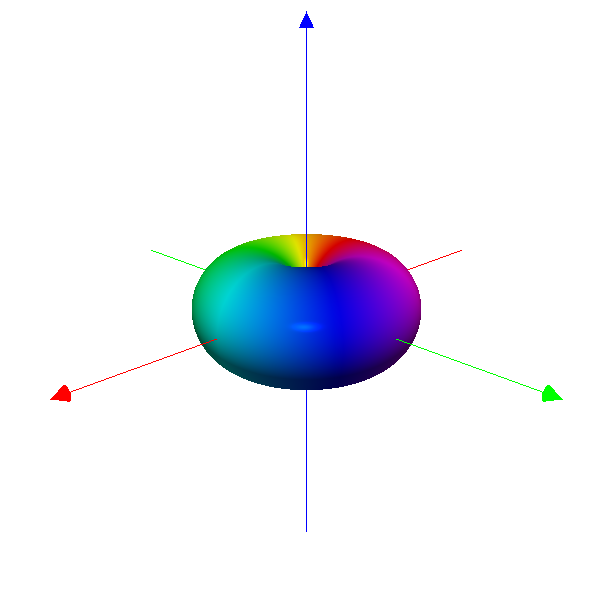
\includegraphics[width=0.15\textwidth,trim={0 3cm 0 -2cm},clip]{1p1} & \\
  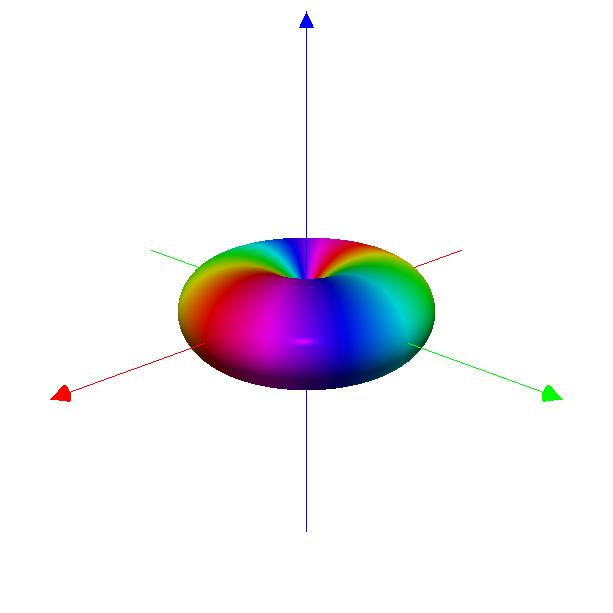
\includegraphics[width=0.15\textwidth,trim={0 3cm 0 -2cm},clip]{2m2} & 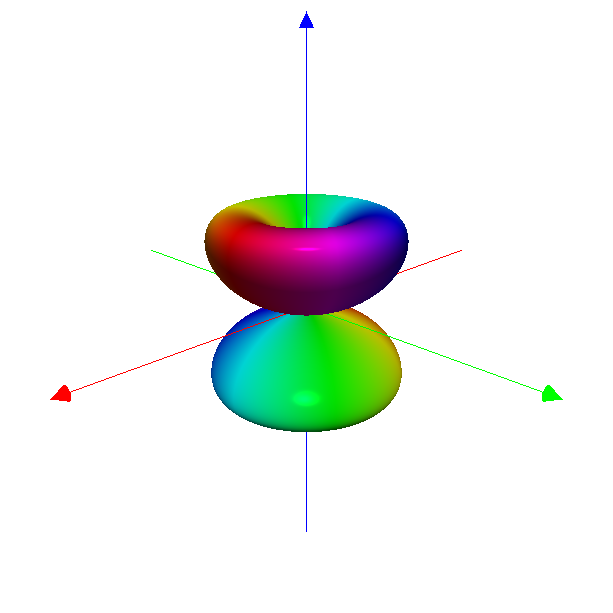
\includegraphics[width=0.15\textwidth,trim={0 3cm 0 -2cm},clip]{2m1} & 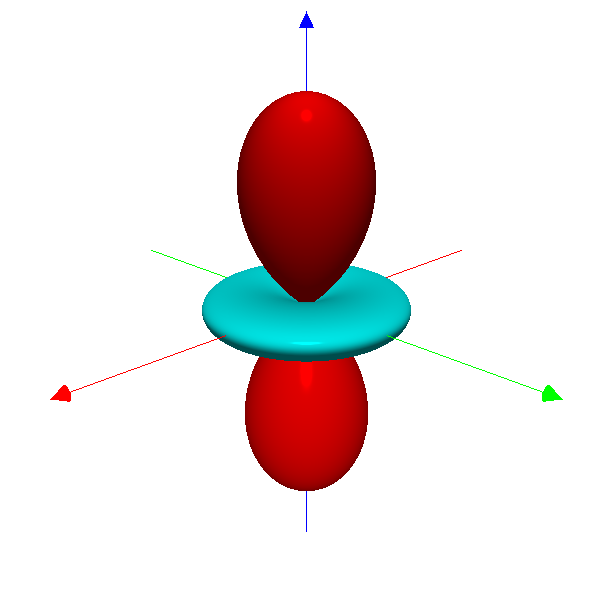
\includegraphics[width=0.15\textwidth,trim={0 3cm 0 -2cm},clip]{20} & 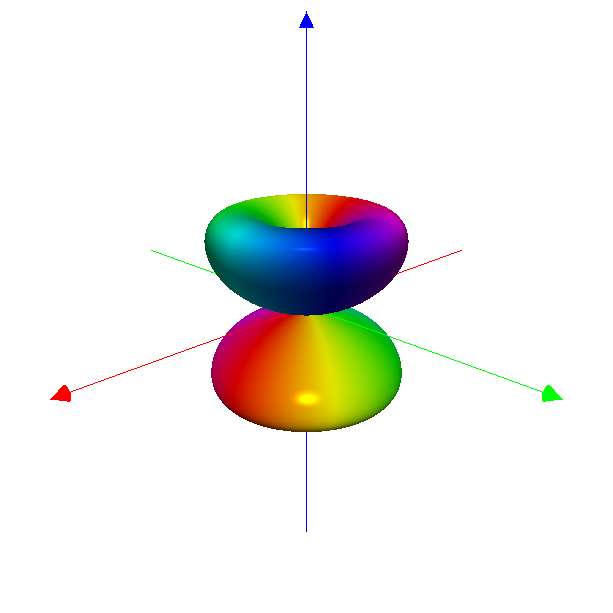
\includegraphics[width=0.15\textwidth,trim={0 3cm 0 -2cm},clip]{2p1} & 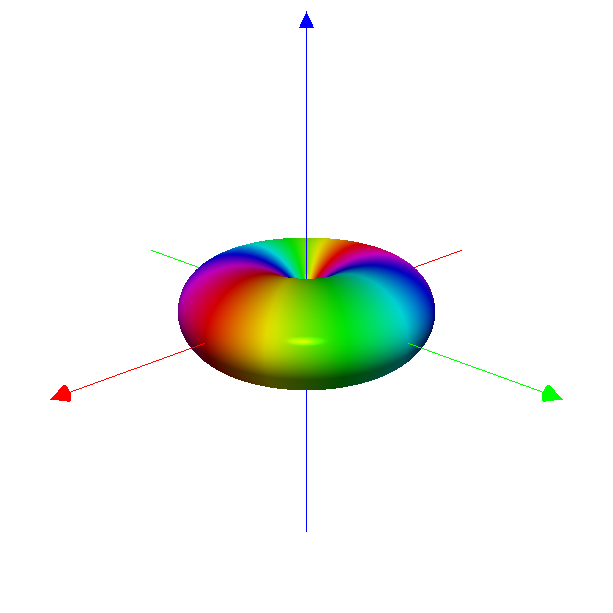
\includegraphics[width=0.15\textwidth,trim={0 3cm 0 -2cm},clip]{2p2}
  \end{tabular}
  \end{center}
  
  \Put(180,250){\emph{
  $\boxed{\begin{aligned}
  & \text{Spherical harmonics: } Y_{lm}(\theta,\phi) \\
  & l = 0,1,\ldots \qquad m = -l,\ldots,l
  \end{aligned}}$}}
\end{frame}

\begin{frame}[t]
  \frametitle{One-electron problem}
  \footnotesize
  Define $u(r) \equiv rR(r)$, \emph{radial equation}
  \[\boxed{-\frac{1}{2} \frac{d^2u}{dr^2} + \left[ V(r) + \frac{l(l+1)}{2r^2} \right] u = E u}\]
  where $V(r)=-Z/r$
  \pause
  \setcounter{subfigure}{0}
  \begin{figure}[h!]
  \centering
  \subfloat[][$Z=1$]{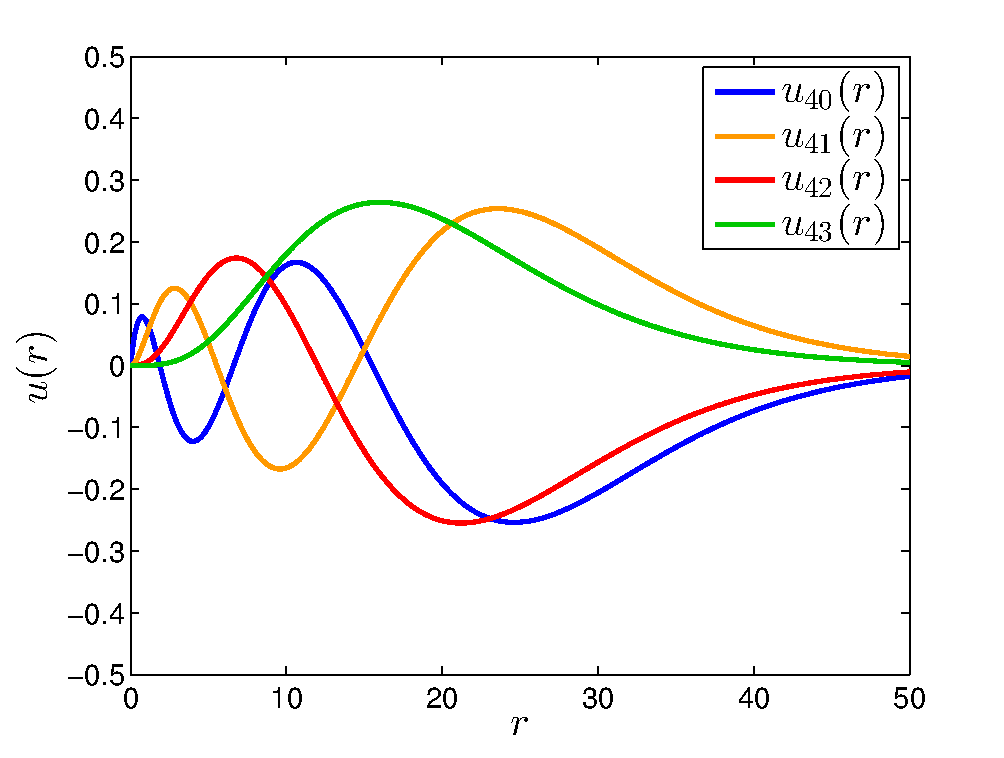
\includegraphics[width=0.325\textwidth]{Z1}}
  \subfloat[][$Z=2$]{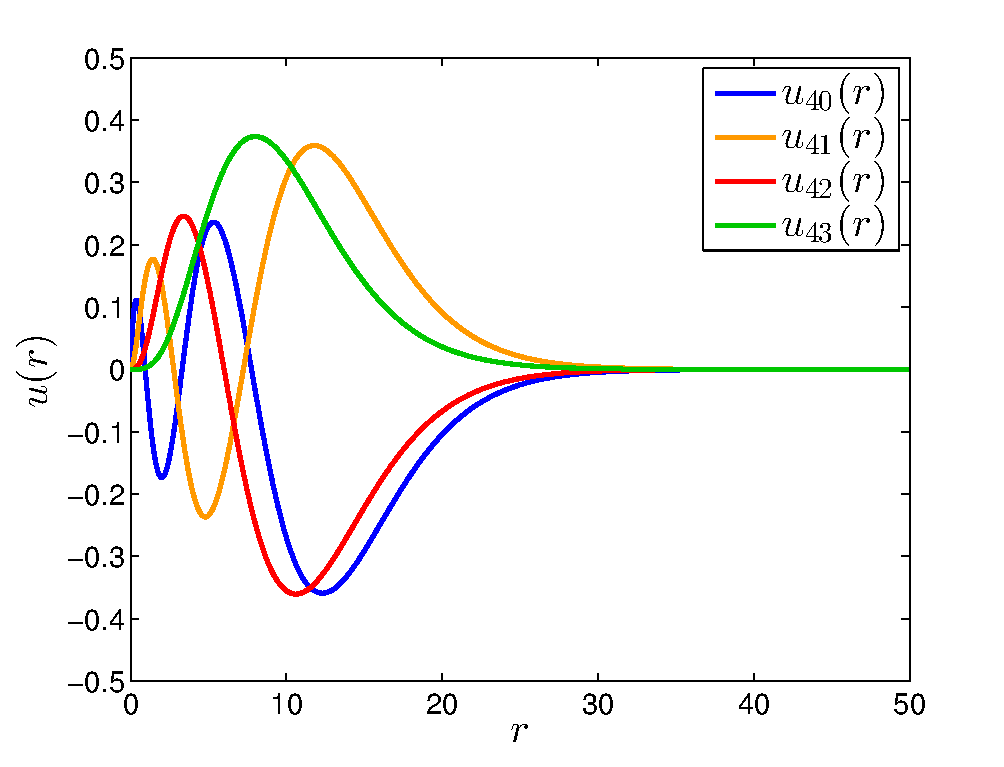
\includegraphics[width=0.325\textwidth]{Z2}}
  \subfloat[][$Z=3$]{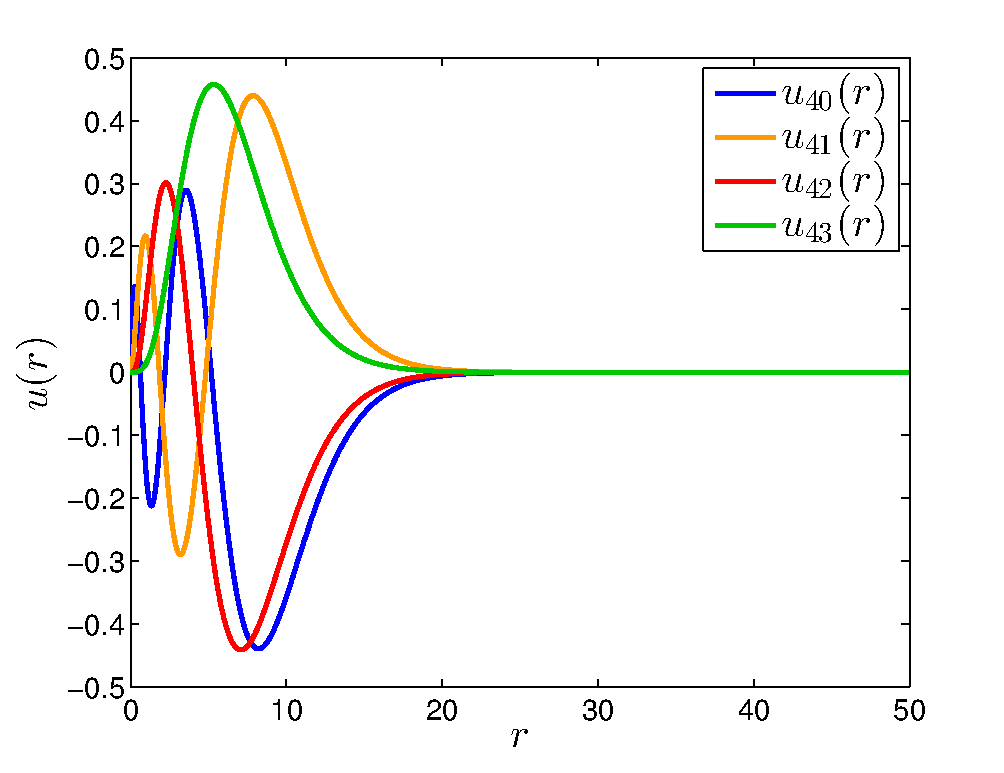
\includegraphics[width=0.325\textwidth]{Z3}}
  \end{figure}
\end{frame}

\begin{frame}[t]
  \frametitle{Logarithmic grid}
  \footnotesize
  Construct a \emph{logarithmic} grid,
  $ 0 < r_0 < \cdots < r_{n-1} < \infty $, where
  \[r_i = \frac{1}{Z} e^{x_i}\]
  \begin{center}
  \setlength{\unitlength}{5pt}
  \begin{picture}(53.6518,0)
  \put(0,0){\line(1,0){53.6518}}
  \put(0,0){\line(0,1){1}}
  \put(0.2216,0){\line(0,1){1}}
  \put(0.4923,0){\line(0,1){1}}
  \put(0.8229,0){\line(0,1){1}}
  \put(1.2268,0){\line(0,1){1}}
  \put(1.7200,0){\line(0,1){1}}
  \put(2.3224,0){\line(0,1){1}}
  \put(3.0583,0){\line(0,1){1}}
  \put(3.9570,0){\line(0,1){1}}
  \put(5.0547,0){\line(0,1){1}}
  \put(6.3954,0){\line(0,1){1}}
  \put(8.0330,0){\line(0,1){1}}
  \put(10.0332,0){\line(0,1){1}}
  \put(12.4762,0){\line(0,1){1}}
  \put(15.4601,0){\line(0,1){1}}
  \put(19.1046,0){\line(0,1){1}}
  \put(23.5561,0){\line(0,1){1}}
  \put(28.9931,0){\line(0,1){1}}
  \put(35.6339,0){\line(0,1){1}}
  \put(43.7449,0){\line(0,1){1}}
  \put(53.6518,0){\line(0,1){1}}
  \put(-0.5,-2){$r_0$}
  \put(53.1518,-2){$r_{n-1}$}
  \end{picture}
  \end{center}
  and $x$ is a \emph{uniformly} distributed grid
  \[ x_i = x_0 + i \Delta x \]
  \begin{center}
  \setlength{\unitlength}{5pt}
  \begin{picture}(53.6520,0)
  \put(0,0){\line(1,0){53.6520}}
  \put(0,0){\line(0,1){1}}
  \put(2.6826,0){\line(0,1){1}}
  \put(5.3652,0){\line(0,1){1}}
  \put(8.0478,0){\line(0,1){1}}
  \put(10.7304,0){\line(0,1){1}}
  \put(13.4130,0){\line(0,1){1}}
  \put(16.0956,0){\line(0,1){1}}
  \put(18.7782,0){\line(0,1){1}}
  \put(21.4608,0){\line(0,1){1}}
  \put(24.1434,0){\line(0,1){1}}
  \put(26.8260,0){\line(0,1){1}}
  \put(29.5086,0){\line(0,1){1}}
  \put(32.1912,0){\line(0,1){1}}
  \put(34.8738,0){\line(0,1){1}}
  \put(37.5564,0){\line(0,1){1}}
  \put(40.2390,0){\line(0,1){1}}
  \put(42.9216,0){\line(0,1){1}}
  \put(45.6042,0){\line(0,1){1}}
  \put(48.2868,0){\line(0,1){1}}
  \put(50.9694,0){\line(0,1){1}}
  \put(53.6520,0){\line(0,1){1}}
  \put(-0.5,-2){$x_0$}
  \put(53.1520,-2){$x_{n-1}$}
  \end{picture}
  \end{center}
\end{frame}

\begin{frame}[t]
  \frametitle{Logarithmic grid}
  \footnotesize
  \setcounter{subfigure}{0}
  \begin{figure}[h!]
  \centering
  \subfloat[][$Z=1$]{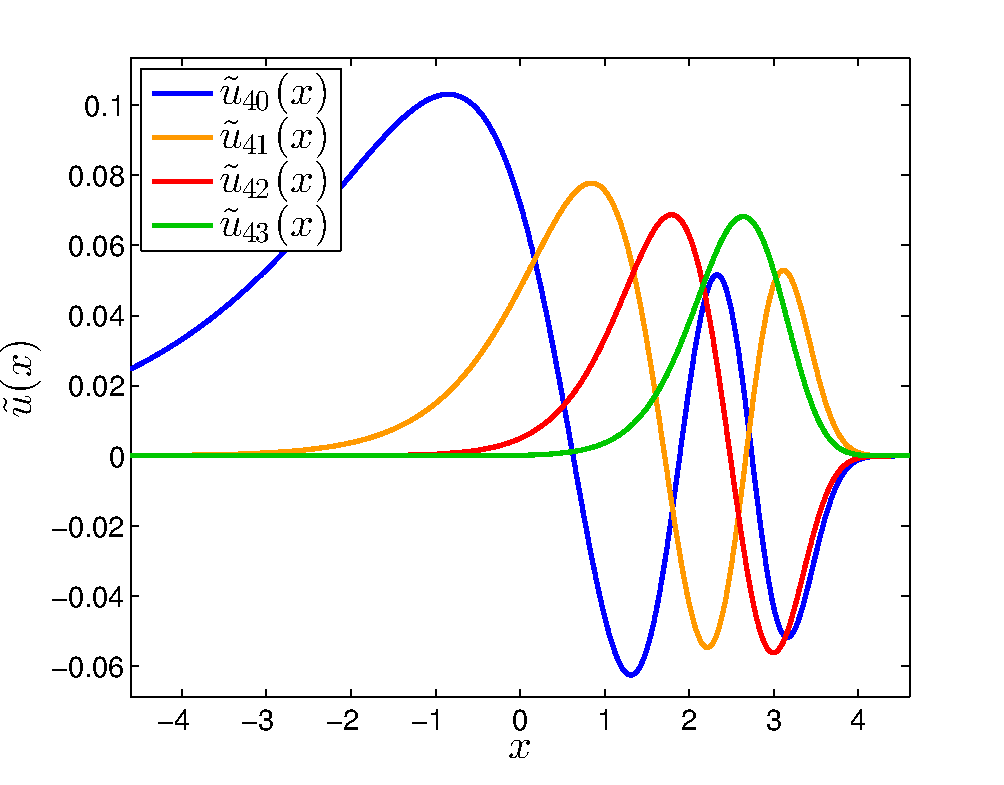
\includegraphics[width=0.325\textwidth]{Z1t}}
  \subfloat[][$Z=2$]{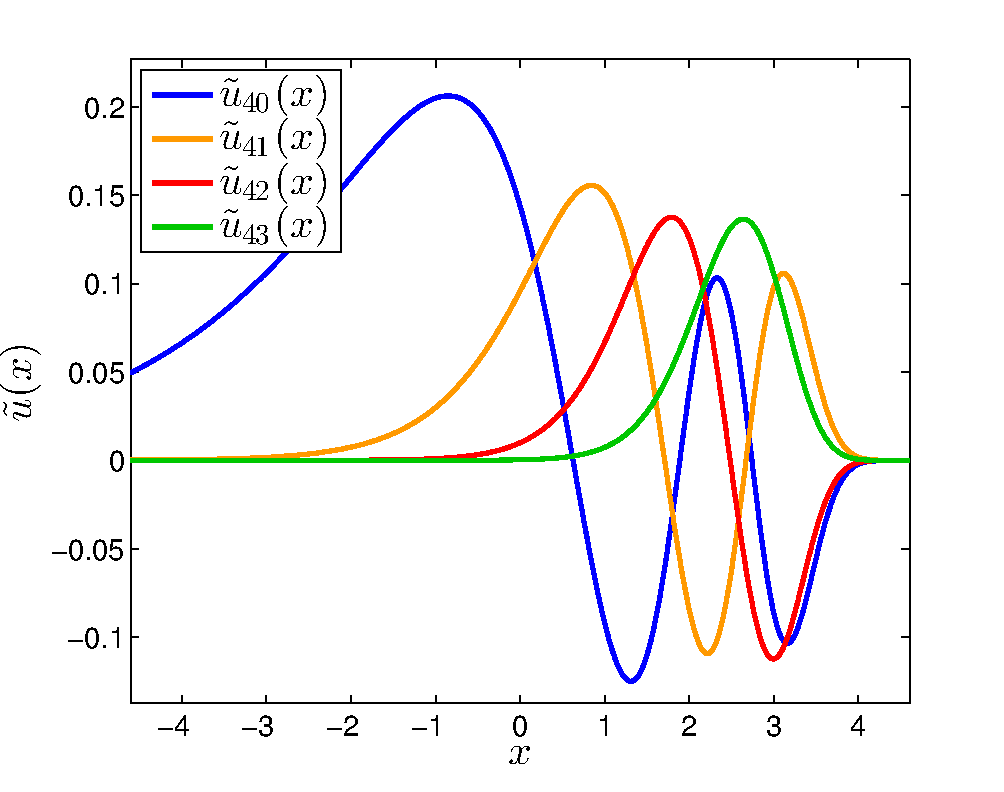
\includegraphics[width=0.325\textwidth]{Z2t}}
  \subfloat[][$Z=3$]{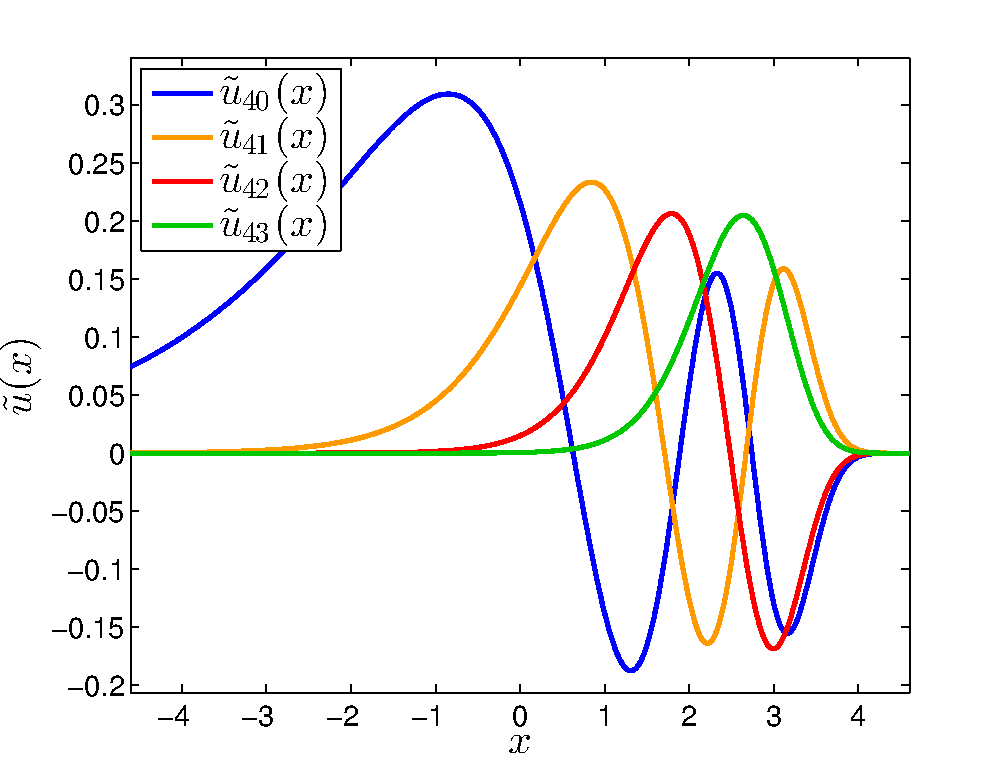
\includegraphics[width=0.325\textwidth]{Z3t}}
  \end{figure}
  Rescale $\tilde{u} \equiv u/\sqrt{r}$, the \emph{transformed radial equation}
  \[ -\frac{1}{2} \frac{d^2\tilde{u}}{dx^2} + \left[ r^2 V(r) + \frac{1}{2} \Big(l+\frac{1}{2}\Big)^2 \right] \tilde{u} = r^2 E \tilde{u} \]
\end{frame}


% \begin{frame}[t]
%   \frametitle{Numerov's method}
%   \footnotesize
%   Finite difference
%   \[\frac{d^2\tilde{u}}{dx^2} = \frac{\tilde{u}_{i+1} - 2\tilde{u}_i + \tilde{u}_{i-1}}{\Delta x^2} + \mathcal{O}(\Delta x^2)\]
%   \pause
%   \emph{Numerov's method}
%   \[\frac{d^2\tilde{u}}{dx^2} = \frac{\tilde{u}_{i+1} - 2\tilde{u}_i + \tilde{u}_{i-1}}{\Delta x^2} - \frac{1}{12}\frac{\tilde{u}_{i+1}^{''} - 2\tilde{u}_i^{''} + \tilde{u}_{i-1}^{''}}{\Delta x^2}\Delta x^2 + \mathcal{O}(\Delta x^4)\]
%   \pause
%   Use the original ODE
%   \[\tilde{u}_i^{''} = -2 k_i^2 \tilde{u_i}
%   \quad \text{and} \quad k_i^2 \equiv r_i^2 E - r_i^2 V(r_i) - \frac{1}{2} \Big(l+\frac{1}{2}\Big)^2\]
%   \pause
%   3-point \alert{recursion}!
%   \[\tilde{u}_{i\pm1} = \frac{(2-\frac{5\Delta x^2}{3}k_i^2)\tilde{u}_i - (1+\frac{\Delta x^2}{6}k_{i\mp1}^2)\tilde{u}_{i\mp1}}{1+\frac{\Delta x^2}{6}k_{i\pm1}^2}\]
% \end{frame}

\begin{frame}[t]
  \frametitle{The shooting and matching methods}
  \footnotesize
%   \begin{tabular}{|c|c|}
%     \hline
%     & Initialization \\ \hline
%     Forward &
%     $\begin{aligned}
%     \smash[b]{\vphantom{\Big|}}
%     \tilde{u}_0 & = r_0^{l+1} / \sqrt{r_0} \\
%     \tilde{u}_1 & = r_1^{l+1} / \sqrt{r_1}
%     \smash[t]{\vphantom{\Big|}}
%     \end{aligned}$ \\ \hline
%     Backward &
%     $\begin{aligned}
%     \smash[b]{\vphantom{\Big|}}
%     \tilde{u}_{n-1} & = e^{-\beta r_{n-1}} / \sqrt{r_{n-1}} \\
%     \tilde{u}_{n-2} & = e^{-\beta r_{n-2}} / \sqrt{r_{n-2}}
%     \smash[t]{\vphantom{\Big|}}
%     \end{aligned}$ \\
%     \hline
%   \end{tabular}
  \emph{Numerov's method}
  
  \vspace{1em}
  $\tilde{u}_{i\pm1} = \dfrac{(2-\frac{5\Delta x^2}{3}k_i^2)\tilde{u}_i - (1+\frac{\Delta x^2}{6}k_{i\mp1}^2)\tilde{u}_{i\mp1}}{1+\frac{\Delta x^2}{6}k_{i\pm1}^2}$
  \Put(5,0){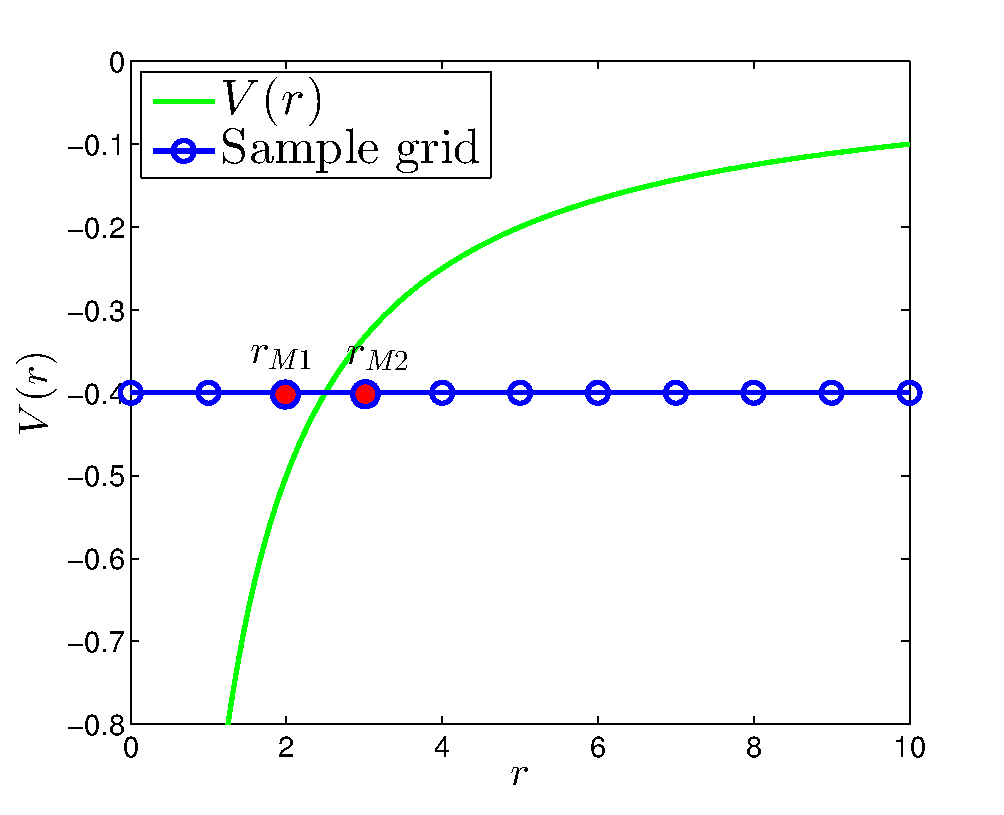
\includegraphics[width=0.4\textwidth]{r1r2}} \pause
  
  \vspace{4em}
  \setcounter{subfigure}{0}
  \begin{figure}[h!]
  \centering
  \subfloat[][$E=-0.6$]{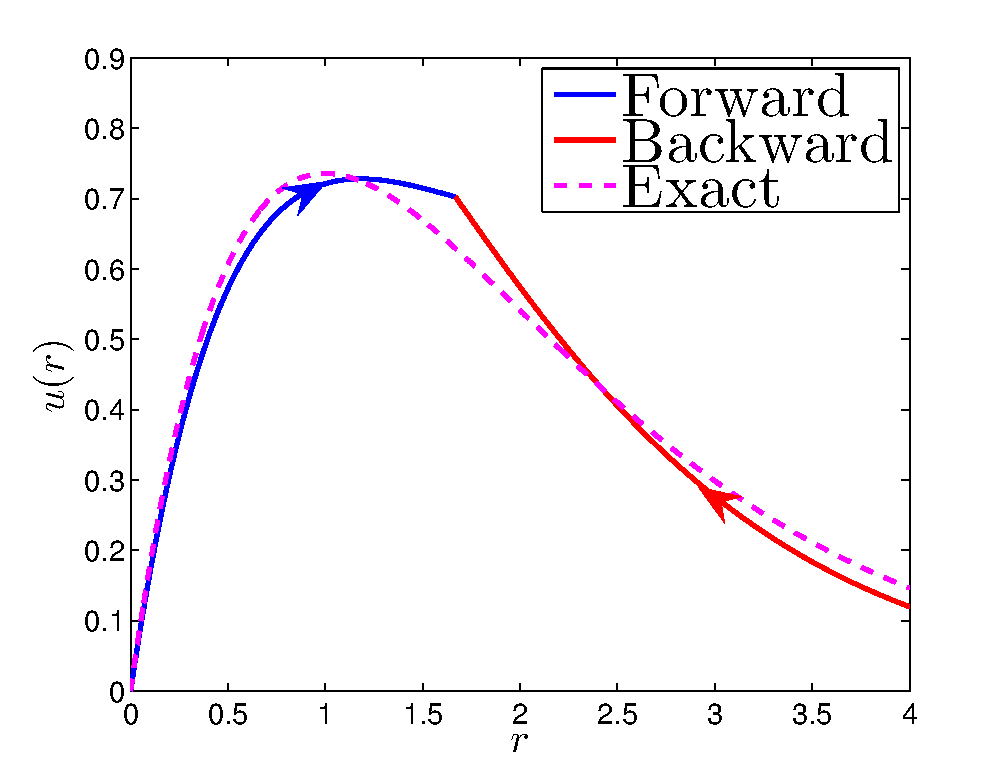
\includegraphics[width=0.325\textwidth]{E06}} \pause
  \subfloat[][$E=-0.4$]{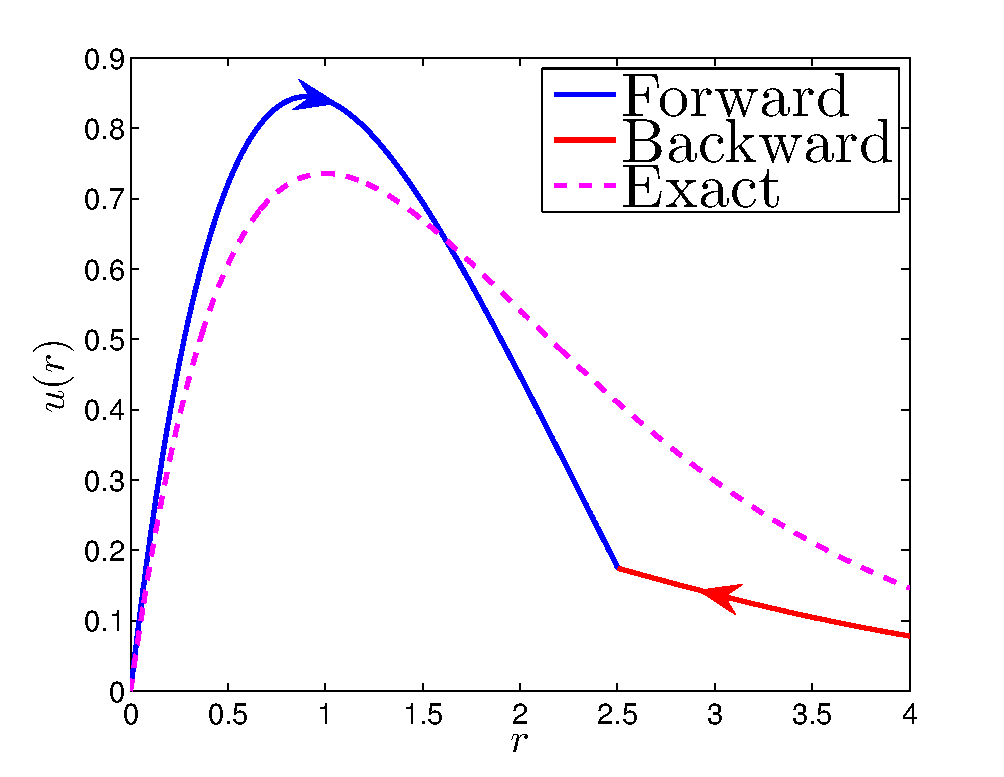
\includegraphics[width=0.325\textwidth]{E04}} \pause
  \subfloat[][$E=-0.5$]{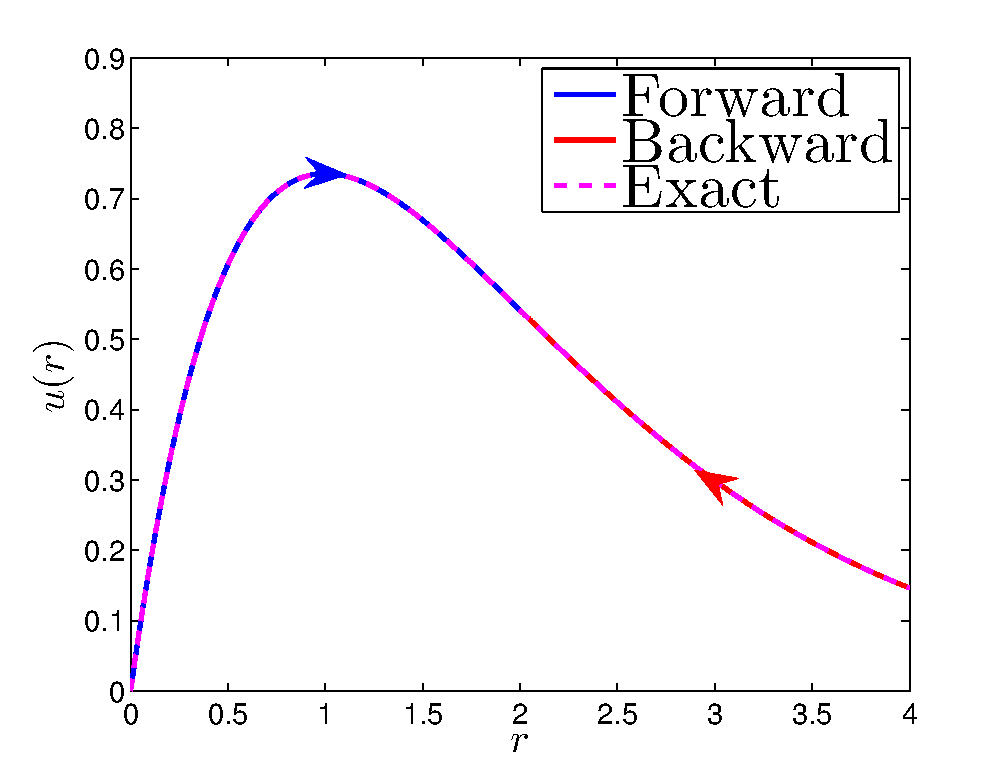
\includegraphics[width=0.325\textwidth]{E05}}
  \end{figure}
\end{frame}

\begin{frame}[t]
  \frametitle{Numerical and exact eigen-energy comparison}
  \footnotesize
  \centering
  \begin{tabular}{ c | c | r | r | r | r }
    \hline
  Elem & Orbital & Numerical & Exact & Abs Error & Rel Error \\ \hline \hline
    H &  $1s$  &  $-0.500000$  &  $-0.500000$  &  0.000000  &  0.000000 \\  \hline
    C &  $1s$  &  $-18.000002$  &  $-18.000000$  &  0.000002  &  0.000000 \\ 
      &  $2s$  &  $-4.499999$  &  $-4.500000$  &  0.000001  &  0.000000 \\ 
      &  $2p$  &  $-4.500001$  &  $-4.500000$  &  0.000001  &  0.000000 \\  \hline
  Fe &  $1s$  &  $-338.000032$  &  $-338.000000$  &  0.000032  &  0.000000 \\ 
      &  $2s$  &  $-84.499984$  &  $-84.500000$  &  0.000016  &  0.000000 \\ 
      &  $2p$  &  $-84.500012$  &  $-84.500000$  &  0.000012  &  0.000000 \\ 
      &  $3s$  &  $-37.555556$  &  $-37.555556$  &  0.000000  &  0.000000 \\ 
      &  $3p$  &  $-37.555556$  &  $-37.555556$  &  0.000000  &  0.000000 \\
      &  $3d$  &  $-37.555555$  &  $-37.555556$  &  0.000001  &  0.000000 \\
      &  $4s$  &  $-21.125000$  &  $-21.125000$  &  0.000000  &  0.000000 \\
    \hline
  \end{tabular}
  
  \emph{\[\boxed{\text{One electron only!}}\]}
\end{frame}
